%!TEX encoding = UTF-8 Unicode
%!TEX root = ../lect-week07.tex

%%%


%\begin{Slide}{TODO: Begrepp att förklara}
%  Tänk igenom ordningen:
%  \begin{itemize}
%    \item OO, arv, supertyp, subtyp, bastyp, polymorfism, ... 
%  \end{itemize}
%\end{Slide}


\Subsection{Överskugging}

\begin{Slide}{Medlemmar, arv och överskuggning}\SlideFontTiny
\begin{multicols}{2}
Olika sorters överskuggningsbara medlemmar i klasser och traits i \Emph{Scala}:
\begin{itemize}
\item \code{def}
\item \code{val}
\item \code{lazy val}
\item \code{var}
\end{itemize}


\columnbreak

\pause

Olika sorters överskuggningsbara instansmedlemmar i \Emph{Java}:
\begin{itemize}
\item variabel 
\item metod
\end{itemize}

{\SlideFontTiny Medlemmar som är \jcode{static} kan ej överskuggas (men döljas) vid arv.}

\vspace{0.5em}
\end{multicols}

\pause
\begin{itemize}\SlideFontTiny
\item När man överskuggar \Eng{override} en medlemmen med en annan medlem med samma namn i en subtyp, får denna medlem en (ny) implementation. 

\item När man konstruerar ett objektorienterat språk gäller det att man definierar sunda överskuggningsregler vid arv. Detta är förvånansvärt knepigt.

\item Singelobjekt kan ej ärvas (och medlemmar i singelobjekt kan därmed ej överskuggas).
\end{itemize}
\end{Slide}


\begin{Slide}{Fördjupning: Regler för överskuggning i Scala} \SlideFontTiny
\label{slideW07:overriderules}
En medlem M1 i en supertyp får överskuggas av en medlem M2 i en subtyp, enligt dessa regler:
\begin{enumerate}
\item M1 och M2 ska ha samma namn och typerna ska matcha.
\item \code{def} får bytas ut mot: \code{def}, \code{val}, \code{var}, \code{lazy val}
\item \code{val} får bytas ut mot: \code{val}, och om M1 är abstrakt mot en \code{lazy val}.
\item \code{var} får bara bytas ut mot en \code{var}.
\item \code{lazy val} får bara bytas ut mot en \code{lazy val}.
\item Om en medlem i en supertyp är abstrakt \emph{behöver} man inte använda nyckelordet \code{override} i subtypen. (Men det är bra att göra det ändå så att kompilatorn hjälper dig att kolla att du verkligen överskuggar något.) 
\item Om en medlem i en supertyp är konkret \emph{måste} man använda nyckelordet \code{override} i subtypen, annars ges kompileringsfel.
\item M1 får inte vara \code{final}.
\item M1 får inte vara \code{private} eller \code{private[this]}, men kan vara \code{private[X]} om M2 också är \code{private[X]}, eller \code{private[Y]} om X innehåller Y.   
\item Om M1 är \code{protected} måste även M2 vara det.

\end{enumerate}
\end{Slide}

\ifkompendium\else
\begin{Slide}{Fördjupning: Regler för överskuggning i Java}
\url{http://docs.oracle.com/javase/tutorial/java/IandI/override.html}
\end{Slide}
\fi

\Subsection{Trait eller abstrakt klass?}

\begin{Slide}{Trait eller abstrakt klass?} 
\SlideFontSmall
\label{slideW07:traitorclass}
\begin{multicols}{2}
Använd en \Emph{trait} som supertyp om...
\begin{itemize}
\item ...du är osäker på vilket som är bäst. (Du kan alltid ändra till en abstrakt klass senare.)
\item ...du vill kunna mixa in din trait tillsammans med andra traits.
\item ...du bara har abstrakta medlemmar. 
\end{itemize}

\columnbreak

Använd en \Alert{abstract class} som supertyp om...
\begin{itemize}
\item ...du vill ge supertypen en parameter vid konstruktion.
\item ...du vill ärva supertypen från klasser skrivna i Java.
\item ...du vill minimera vad som behöver omkompileras vid ändringar. 
\end{itemize}


\end{multicols}
\end{Slide}


\Subsection{\texttt{super}}

\begin{Slide}{\texttt{super}}
\begin{REPL}
scala> class X { def gurka = "super pepinos" }

scala> class Y extends X { override def gurka = ":("; def sup = super.gurka }

scala> val y = new Y
y: Y = Y@26ba2a48

scala> y.gurka
res0: String = :(
\end{REPL}

\pause
\begin{REPLnonum}
scala> y.sup
res1: String = super pepinos

\end{REPLnonum}


\pause
\begin{tikzpicture}[overlay]
     \node at (7.5,1.5) {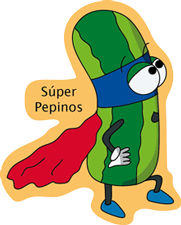
\includegraphics[scale=0.5]{../img/ttsuper}};
\end{tikzpicture}

\end{Slide}


%\begin{Slide}{Designexempel: Klassen ???}\small
%TODO:
%  \begin{itemize} 
%  \item 
%  \end{itemize}
%\end{Slide}










